\documentclass[a4paper,12pt]{article}
\usepackage[a4paper,top=1.3cm,bottom=2cm,left=1.5cm,right=1.5cm,marginparwidth=0.75cm]{geometry}
\usepackage{cmap}
\usepackage{mathtext}
\usepackage[T2A]{fontenc}
\usepackage[utf8]{inputenc}
\usepackage[english,russian]{babel}
\usepackage{siunitx}

\usepackage{graphicx}

\usepackage{wrapfig}
\usepackage{tabularx}
\usepackage{multirow}

\usepackage{hyperref}
\usepackage[rgb]{xcolor}
\hypersetup{
colorlinks=true,urlcolor=blue
}
\usepackage{amsmath,amsfonts,amssymb,amsthm,mathtools}
\usepackage{icomma}
\mathtoolsset{showonlyrefs=false}
\usepackage{euscript}
\usepackage{mathrsfs}
\DeclareMathOperator{\sgn}{\mathop{sgn}}
\newcommand*{\hm}[1]{#1\nobreak\discretionary{}
{\hbox{$\mathsurround=0pt #1$}}{}}

%%% Заголовок
\author{Макаров Лев Евгеньевич}
\title{Лабораторная работа №3.4.1

Диа- и парамагнетики
}
\date{\today}

\begin{document}

\begin{titlepage}
	\begin{center}
		{\large МОСКОВСКИЙ ФИЗИКО-ТЕХНИЧЕСКИЙ ИНСТИТУТ (НАЦИОНАЛЬНЫЙ ИССЛЕДОВАТЕЛЬСКИЙ УНИВЕРСИТЕТ)}
	\end{center}
	\begin{center}
		{\large Физтех-школа фотоники, электроники и молекулярной физики}
	\end{center}
	
	
	\vspace{4.5cm}
	{\huge
		\begin{center}
			{\bf Отчёт о выполнении лабораторной работы 3.4.1}\\
			Диа- и парамагнетики
		\end{center}
	}
	\vspace{2cm}
	\begin{flushright}
		{\LARGE Автор:\\ Макаров Лев Евгеньевич \\
			\vspace{0.2cm}
			Б04-306}
	\end{flushright}
	\vspace{8cm}
	\begin{center}
		Долгопрудный 2024
	\end{center}
\end{titlepage}

\section{Введение}

\textbf{Цель работы:} 
\begin{enumerate}
	\item измерение магнитной восприимчивости диа- и парамагнитного образцов
\end{enumerate}

\textbf{В работе используются:} 
\begin{itemize}
    \item электромагнит
    \item аналитические весы
    \item милливеберметр
    \item регулируемый источник постоянного тока
    \item образцы
\end{itemize}
\medskip

\section{Теоретические сведения}

Измерение магнитной восприимчивости материалов будем проводить с помощью расчета силы, действующей на магнетик в магнитном поле. При смещении образца на расстояние $ \Delta l $ внутрь магнитного поля магнитная сила, действующая на него, равна
	
\begin{equation}
    F = \left(\frac{\Delta W_m}{\Delta l}\right)_I,
\end{equation}

где $\Delta W_m$ -- изменение магнитной энергии системы при постоянном токе
в обмотке электромагнита и, следовательно, при постоянной величине
магнитного поля в зазоре.
Магнитная энергия рассчитывается по формуле:

\begin{equation*}
    W_m = \frac{1}{2} \int (\mathbf{H}\mathbf{B})d\,V = \frac{1}{2\mu_0}\int\frac{B^2}{\mu}d\,V
\end{equation*}

\begin{wrapfigure}[10]{l}{0.3\textwidth}
    \centering
    \includegraphics[height = 0.12\textheight]{energy}
    \caption{Перемещение магнетика}
    \label{pic:1}
\end{wrapfigure}


 При смещении образца магнитная энергия меняется только в области зазора (в объёме площади $ S $ и высоты $ \Delta l $), а около верхнего конца стержня остаётся неизменной, поскольку магнитного поля там практически нет. Тогда изменение магнитной энергии будет:

\begin{equation*}
    \Delta W_m = \frac{1}{2\mu_0} \frac{(\mu B)^2}{\mu} S \Delta l - \frac{1}{2\mu_0} B^2 S \Delta l = (\mu - 1) \frac{B^2}{2\mu_0} S \Delta l
\end{equation*}

Следовательно, на образец действует сила

\begin{equation}\label{eq:1}
    F = (\mu - 1)\frac{B^2}{2\mu_0}S = \chi\frac{B^2}{2\mu_0}S  
\end{equation}

Знак силы, действующей на образец, зависит от знака $\chi$: образцы из парамагнитных материалов $(\chi  > 0)$ втягиваются в зазор электромагнита, а диамагнитные образцы $(\chi < 0)$ выталкиваются из него.

\section{Эксперементальная установка}

Схема установки представлена на рис. \ref{pic:2}

\clearpage

\begin{figure}[!h]
    \center
    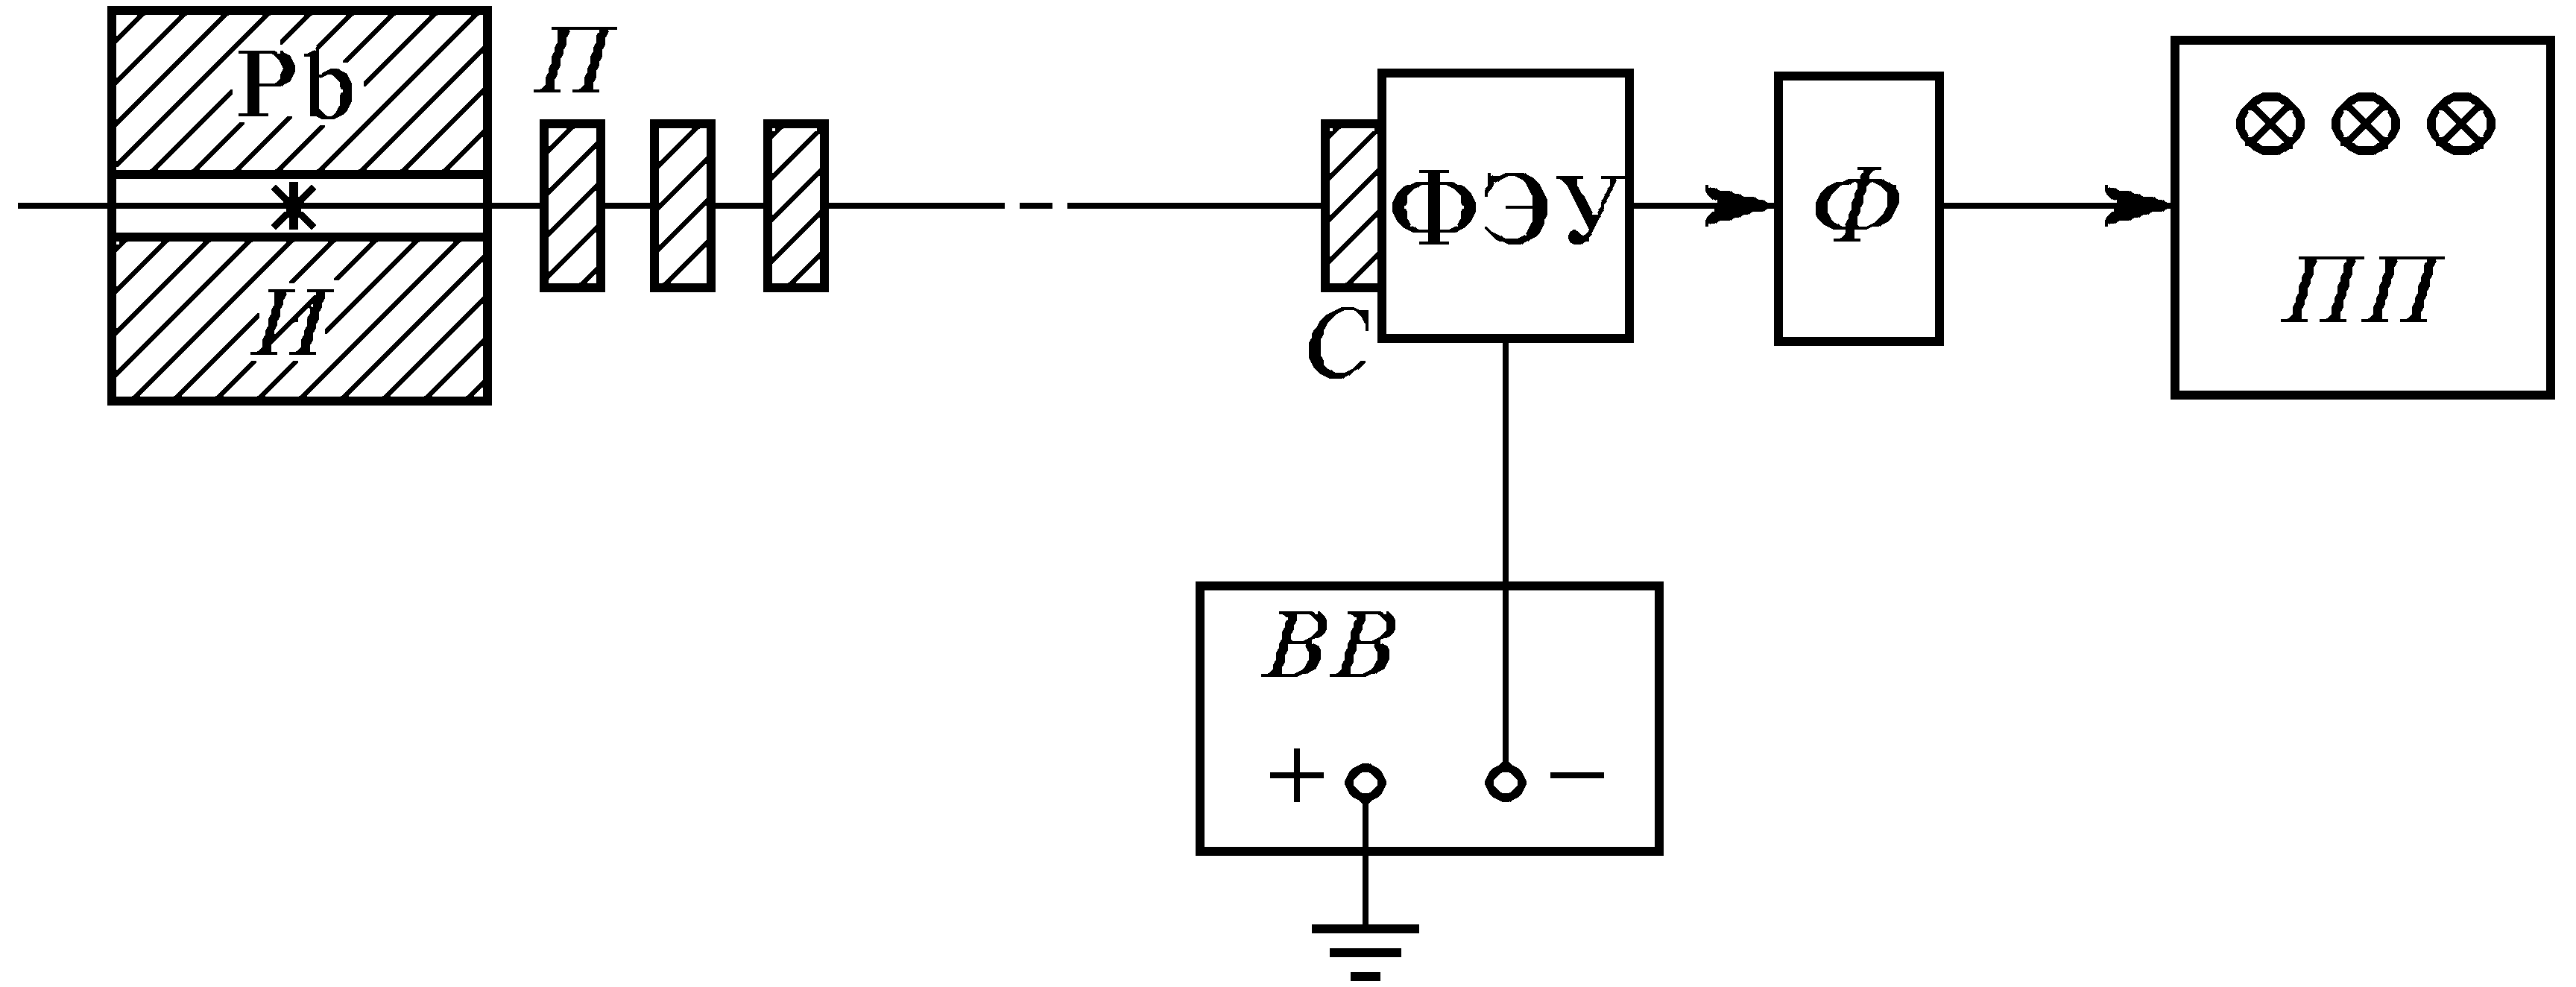
\includegraphics[scale=0.6]{ustan.png}
    \caption{Схема установки}
    \label{pic:2}
\end{figure}

Магнитное поле создаётся в зазоре электромагнита, питаемого постоянным током. Диаметр полюсов существенно превосходит ширину зазора, поэтому поле в средней части зазора однородно. Величина тока, проходящего через обмотки электромагнита, задаётся регулируемым источником питания GPR и измеряется амперметром $А$, встроенным в источник питания. Градуировка электромагнита (связь между индукцией магнитного поля $B$ в зазоре электромагнита и силой тока $I$ в его обмотках) производится при помощи милливеберметра либо тесламетра.
Сила, действующая на образец со стороны магнитного поля измеряется в помощью весов: смотрится разность веса образца вне поля и в поле.

\section{Результаты измерений и обработка данных}

\subsection{Диапазон изменения тока}

Ток через обмотку не превышает $I_{max} = 2,4$ А.

\subsection{Калибровка электромагнита}

При выполнении работы были использованы результаты калибровки предыдущих студентов из-за отсутсвия времени на выполнение.

\subsection{Весы}

Арретируем весы. Весы необходимо арретировать перед каждым изменением тока.

\subsection{Измерение силы на образец}

Подвесим к весам первый образец (алюминиевый) при выключенном электромагните. По весам измерим массу образца: $m_1 = 25252$ мг.

Арретируем весы и проведем измерения силы для нескольких значений тока от минимального к максимальному. Результаты измерений занесем в таблицу \ref{table:1}.

\begin{table}[!ht]
    \centering
    \begin{tabular}{|l|l|l|}
    \hline
        $I$, A & $m$, мг & $F$, мН \\ \hline
        0,30 & 0 & 0 \\ \hline
        0,60 & 2 & 20 \\ \hline
        0,90 & 5 & 49 \\ \hline
        1,20 & 9 & 88 \\ \hline
        1,50 & 13 & 128 \\ \hline
        1,80 & 19 & 186 \\ \hline
        2,10 & 25 & 245 \\ \hline
        2,40 & 31 & 304 \\ \hline
    \end{tabular}\caption{\textit{Зависимость силы от тока для алюминиего образца}}\label{table:1}
\end{table}

Проведем аналогичную серию измерений при уменьшении тока. Результаты запишем в таблицу \ref{table:2}.

\begin{table}[!ht]
    \centering
    \begin{tabular}{|l|l|l|}
    \hline
        $I$, A & $m$, мг & $F$, мН \\ \hline
        2,40 & 33 & 324 \\ \hline
        2,10 & 27 & 265 \\ \hline
        1,80 & 20 & 196 \\ \hline
        1,50 & 14 & 137 \\ \hline
        1,20 & 9 & 88 \\ \hline
        0,90 & 5 & 49 \\ \hline
        0,60 & 2 & 20 \\ \hline
        0,30 & 0 & 0 \\ \hline
    \end{tabular}\caption{\textit{Зависимость силы от тока для алюминиего образца при уменьшении тока}}\label{table:2}
\end{table}

\subsection{Измерение сил для других образцов}

Проведем аналогичные измерения для образцов из вольфрама и графита. Результаты измерений запишем в таблицы \ref{table:3} и \ref{table:4}.

\begin{table}[!ht]
    \centering
    \begin{tabular}{|l|l|l|l|l|l|l|}
    \hline
        $I$, A & $m$, мг & $F$, мН & ~ & $I$, A & $m$, мг & $F$, мН \\ \hline
        0,30 & 2 & 20 & ~ & 2,40 & 112 & 1099 \\ \hline
        0,60 & 8 & 78 & ~ & 2,10 & 93 & 912 \\ \hline
        0,90 & 18 & 177 & ~ & 1,80 & 71 & 697 \\ \hline
        1,20 & 30 & 294 & ~ & 1,50 & 52 & 510 \\ \hline
        1,50 & 47 & 461 & ~ & 1,20 & 34 & 334 \\ \hline
        1,80 & 66 & 647 & ~ & 0,90 & 20 & 196 \\ \hline
        2,10 & 88 & 863 & ~ & 0,60 & 9 & 88 \\ \hline
        2,40 & 112 & 1099 & ~ & 0,30 & 3 & 29 \\ \hline
    \end{tabular}\caption{\textit{Зависимость силы от тока для вольфрамового образца}}\label{table:3}
\end{table}

\begin{table}[!ht]
    \centering
    \begin{tabular}{|l|l|l|l|l|l|l|}
    \hline
        $I$, A & $m$, мг & $F$, мН & ~ & $I$, A & $m$, мг & $F$, мН \\ \hline
        0,30 & 10 & 98 & ~ & 2,40 & 38 & 373 \\ \hline
        0,60 & 22 & 216 & ~ & 2,10 & 44 & 432 \\ \hline
        0,90 & 34 & 334 & ~ & 1,80 & 49 & 481 \\ \hline
        1,20 & 43 & 422 & ~ & 1,50 & 49 & 481 \\ \hline
        1,50 & 47 & 461 & ~ & 1,20 & 46 & 451 \\ \hline
        1,80 & 48 & 471 & ~ & 0,90 & 39 & 383 \\ \hline
        2,10 & 45 & 441 & ~ & 0,60 & 26 & 255 \\ \hline
        2,40 & 38 & 373 & ~ & 0,30 & 14 & 137 \\ \hline
    \end{tabular}\caption{\textit{Зависимость силы от тока для графитового образца}}\label{table:4}
\end{table}

\subsection{Рассчет поля}

Для калибровочных значений тока и потока рассчитаем индукцию магнитного поля и запишем в таблицу \ref{table:5} ($SN = 72 \ \text{см}^2$).

\begin{table}[!ht]
    \centering
    \begin{tabular}{|l|l|l|}
    \hline
        $I$, А & $\Phi$, мВб & $B$, Тл \\ \hline
        0,0 & 1,0 & 0,14 \\ \hline
        0,4 & 1,8 & 0,25 \\ \hline
        0,6 & 2,2 & 0,31 \\ \hline
        1,0 & 3,0 & 0,42 \\ \hline
        1,3 & 3,6 & 0,50 \\ \hline
        1,6 & 4,4 & 0,61 \\ \hline
        2,0 & 5,2 & 0,72 \\ \hline
        2,3 & 5,8 & 0,81 \\ \hline
        2,4 & 5,9 & 0,82 \\ \hline
    \end{tabular}\caption{\textit{Зависимость индукции магнитного поля от тока через электромагнит}}\label{table:5}
\end{table}

Построим градуировочную кривую для электромагнита $B(I)$. Воспользуемся для этого МНК.

\begin{figure}[!ht]
        \centering
	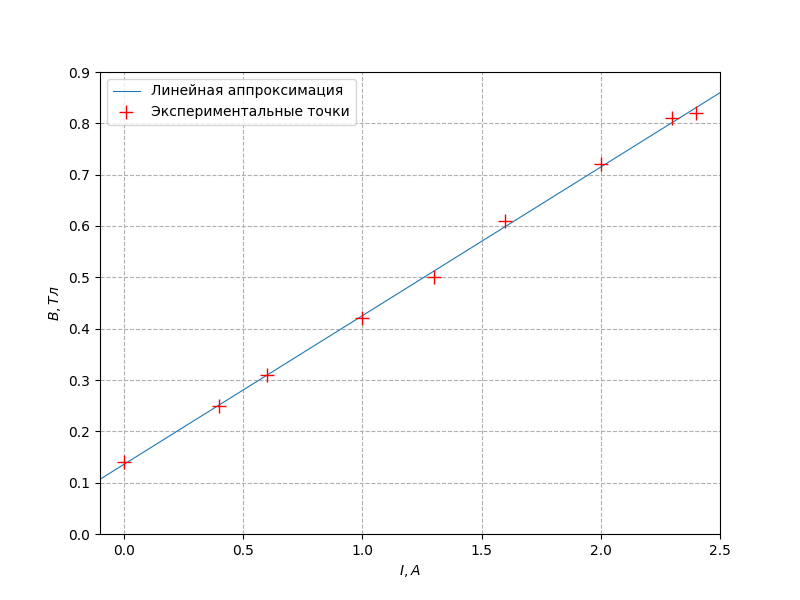
\includegraphics[scale=0.8]{calib_plot.png}
	\caption{\textit{Калибровочная кривая для электромагнита}}
	\label{graph:1}
\end{figure}

Параметры МНК для прямой:

\begin{equation*}
    k = (0,290 \pm 0,003) \ \frac{\text{Тл}}{\text{А}}, \ \ \ b = (0,136 \pm 0,003) \ \text{Тл}
\end{equation*}

Наличие ненулевого $b$ можно объяснить присутствием магнитных помех, создаваемых не элетромагнитом.

\subsection{Зависимость силы от поля}

Построим график зависимости силы от квадрата индукции магнитного поля $F(B^2)$ для всех измерений, согласно формуле \eqref{eq:1} зависимость должна быть линейной, значит можно воспользоваться МНК. Все графики изобразим на рисунке \ref{graph:2}.

\begin{figure}[!ht]
        \centering
	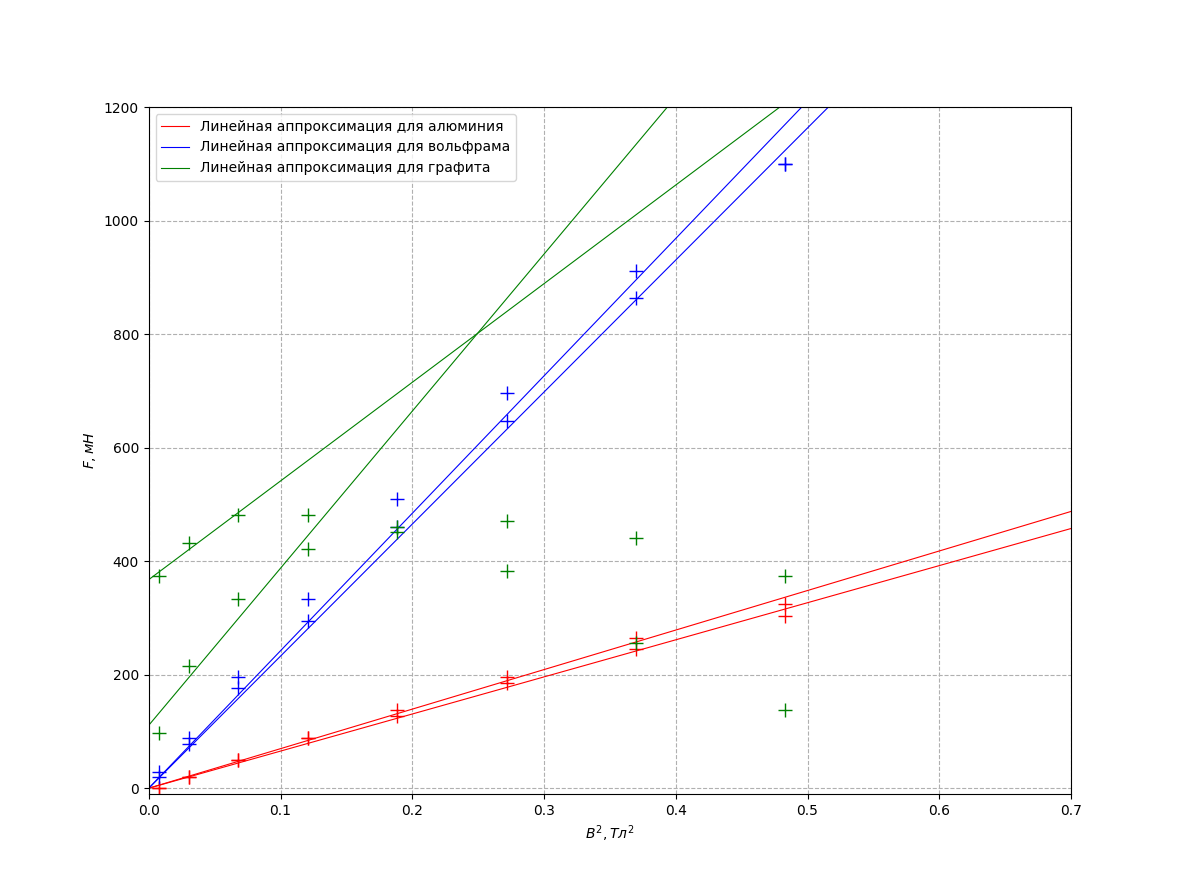
\includegraphics[width=1.0\textwidth]{graph_b2_f.png}
	\caption{\textit{Зависимость силы от квадрата индукции для всех измерений}}
	\label{graph:1}
\end{figure}

Как видно из графика зависимость для графита не выполняется в пределах измерений. Значения коэффициентов наклона:

\begin{equation*}
    k_{Al} = (680 \pm 10) \ \frac{\text{мН}}{\text{Тл}^2} \ \ \ \ \ k_{W} = (2370 \pm 50) \ \frac{\text{мН}}{\text{Тл}^2}
\end{equation*}

Из формулы \eqref{eq:1} найдем магнитную восприимчивость:

\begin{equation*}
    k = \frac{\chi S}{2 \mu_0} \ \implies \ \chi = \frac{2 k \mu_0}{S}
\end{equation*}

Для образцов имеем: $d = (1,000 \pm 0,005)$ см, а значит $S = (0,79 \pm 0,01) \ \text{см}^2$

Отсюда:

\begin{equation*}
    \chi_{Al} = (0,0215 \pm 0,0004) \ \ \ \ \  \chi_{W} = (0,075 \pm 0,002)
\end{equation*}

Полученные значения на порядок отличаются от табличных.

\end{document}